\chapter{Конструкторский раздел}

В данном разделе будут более подробно рассмотрены выбранные в предыдущем разделе методы и алгоритмы, а также предоставлены требования к программному обеспечению.

\section{Требования к программному обеспечению}

Программа должна:
\begin{itemize}
	\item загружать модели из .obj файлов;
	\item визуализировать трехмерные каркасные модели;
	\item визуализировать морфинг двух трехмерных моделей;
	\item преобразовывать модель: поворот, масштабирование и сдвиг;
	\item изменять положение источника света;
	\item изменять положение камеры;
	\item изменять тип вершин, ребер (в режиме морфинга);
	\item изменять размер вершин и ребер (в режиме морфинга).
\end{itemize}


\section{Считывание моделей}

Для задания моделей был выбран один из наиболее популярных и универсальных методов – .obj файлы. 
Рассмотрим этапы считывания данных.
\begin{enumerate}
	\item \textbf{Открытие файла .obj}
	
	Программа открывает файл, предоставляя путь к нему в качестве входного параметра.
	
	\item \textbf{Чтение вершин}
	
	Из файла считываются строки, содержащие координаты вершин. 
	Каждая строка представляет собой набор координат в формате 'v x y z', где x, y и z - координаты вершины.
	
	\item \textbf{Чтение нормалей}
	
	Происходит чтение строк, представляющих нормали. 
	Формат строки - 'vn x y z', где x, y и z создают направление нормали.
	
	\item \textbf{Чтение граней}
	
	Происходит чтение строк, представляющих грани. 
	Формат строки - 'f v1/t1/vn1 v2/t2/vn2...vn/tn/vnn', где 
	\begin{itemize}
		\item v1, v2..vn - индексы вершин, образующих грань;
		\item t1, t2...tn - текстурные координаты;
		\item vn1, vn2...vnn - нормали.
	\end{itemize}
	
	\item \textbf{Обработка и хранение данных}
	
	Прочитанные вершины и грани сохраняются в структуры данных, предназначенные для хранения геометрических данных 
	модели. 
	Вершины сохраняются в массиве, а грани - в структуре, содержащей информацию о связи вершин и порядке их соединения.
	
\end{enumerate}


\section{Общий алгоритм построения изображения}
Рассмотрим алгоритм построения кадра для каркасной модели, он представлен на рисунке~\ref{fig:frame_algo}. 
Для визуализации объектов используется алгоритм Z-буфера представлен на рисунке~\ref{fig:z-buffer}.
Он был рассмотрен для полигонов поверхностной модели.


\begin{figure}[H]
	\centering
	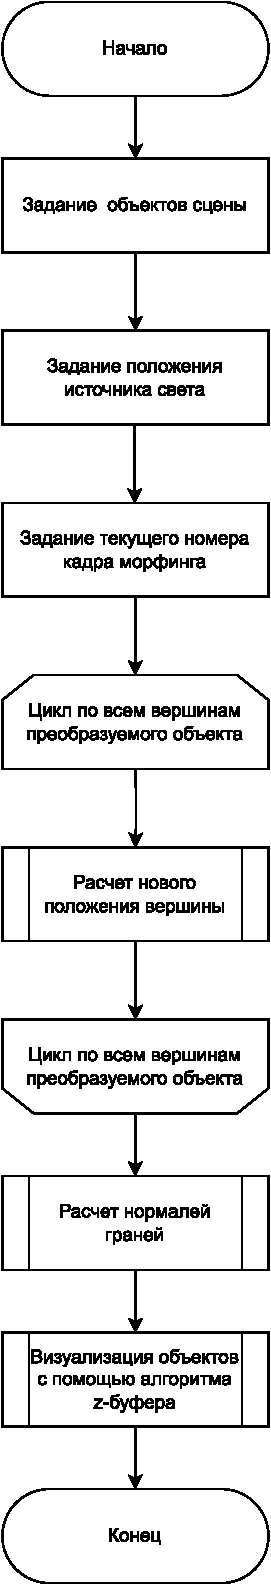
\includegraphics[height=1.45\textwidth]{images/frame_algo_morph.pdf}
	\caption{Общий алгоритм построения кадра}
	\label{fig:frame_algo}
\end{figure}

\begin{figure}[H]
	\centering
	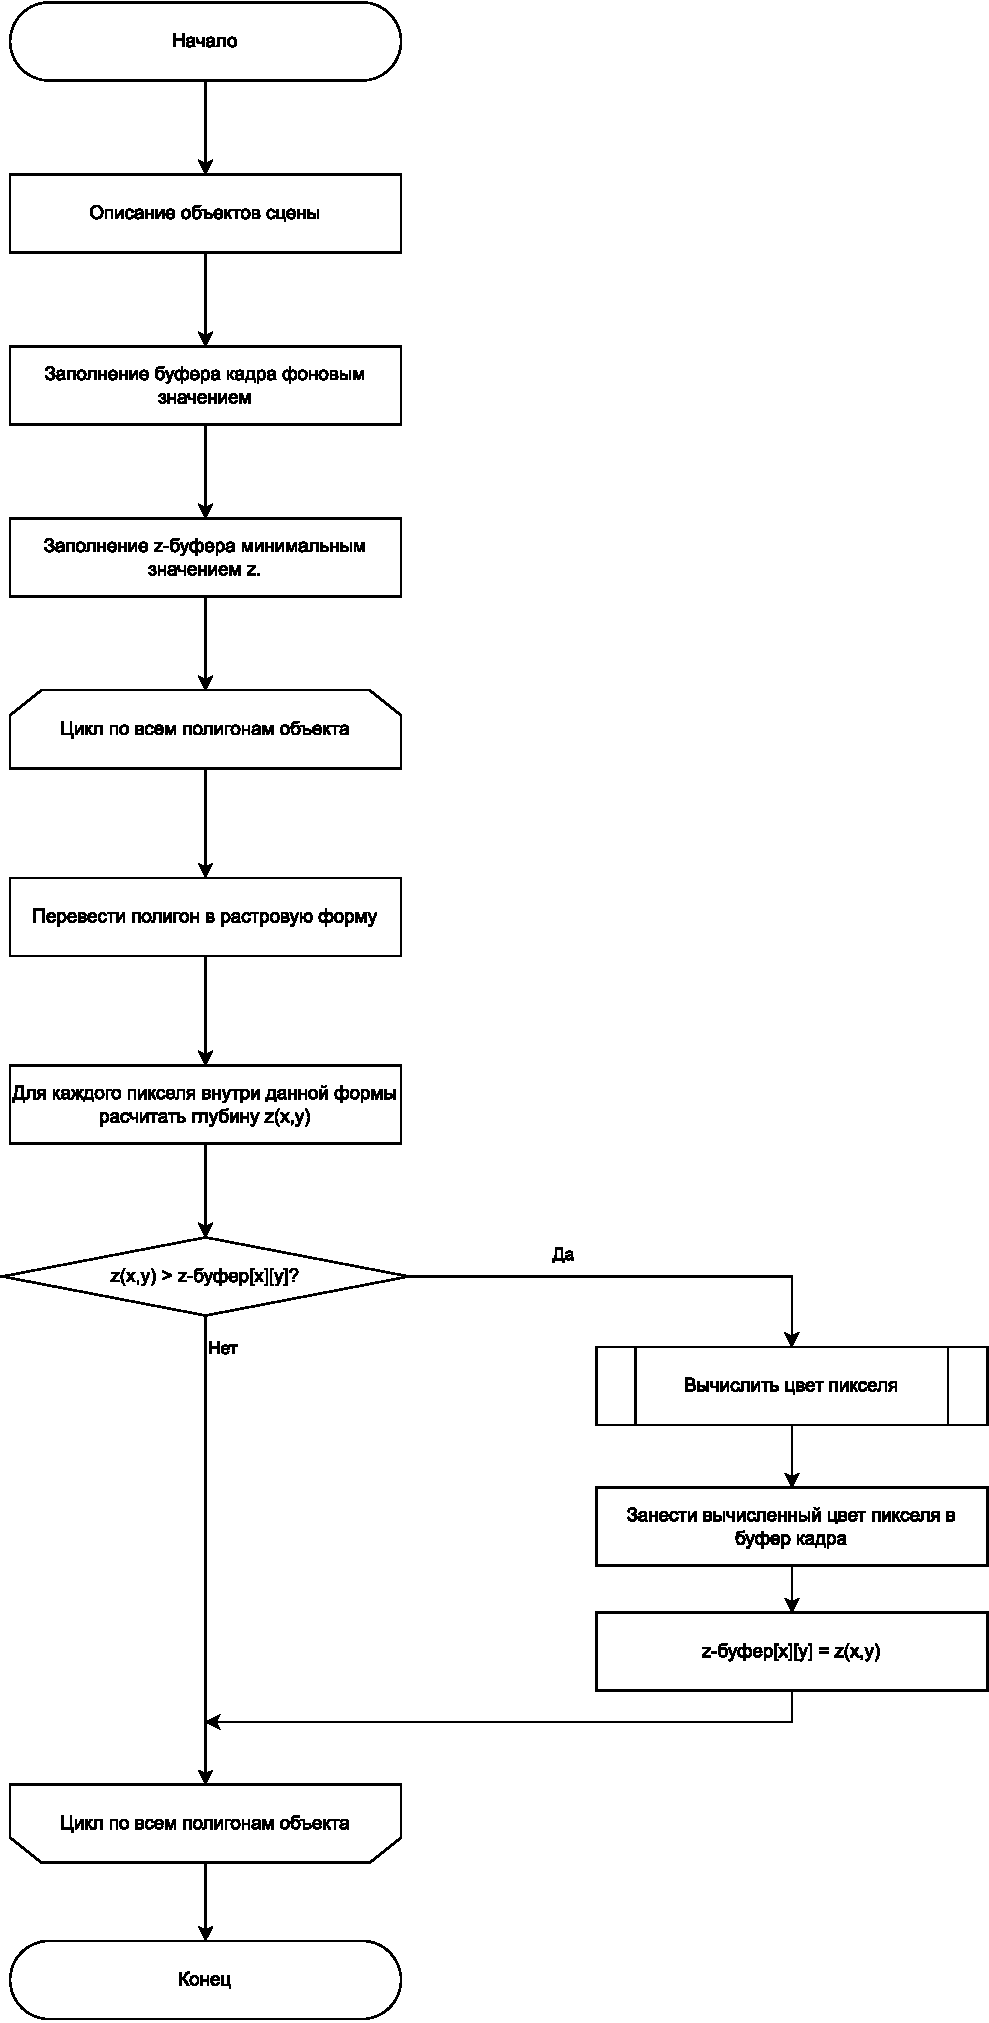
\includegraphics[scale=0.83]{images/z_buffer_morph.pdf}
	\caption{Алгоритм Z-буфера}
	\label{fig:z-buffer}
\end{figure}

\newpage

Математические соображения об алгоритме Гуро приведены в разделе~\ref{sec:draw_algo_analysis}.
Данный алгоритм позволяет получить довольно гладкое изображение при малых вычислительных затратах, что важно при необходимости постоянно пересчета вершин при морфинге.
Необходимо отметить, что интенсивность в вершинах полигона будет определяться как скалярное произведение вектора светового луча (вектора направленного из вершины к источнику света) и нормали в вершине.
\begin{figure}[h]
	\centering
	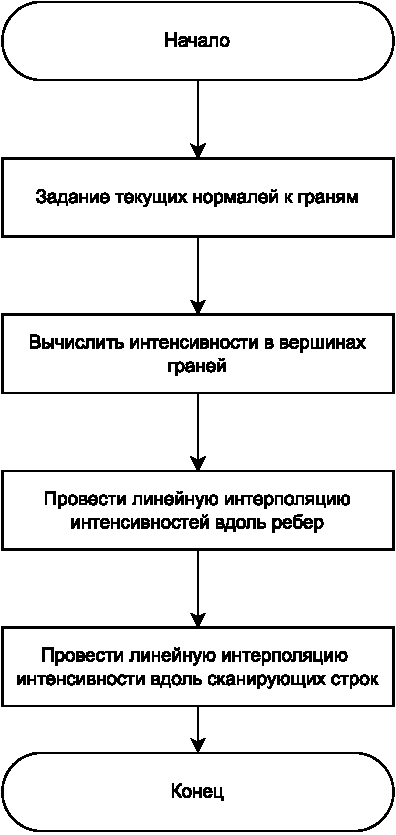
\includegraphics{images/guro_morph.pdf}
	\caption{Алгоритм закраски по Гуро}
	\label{fig:guro_algo}
\end{figure}

\newpage

\section{Алгоритм морфинга}

Рассмотрим алгоритм морфинга двух объектов. Он представлен на рисунке~\ref{fig:morph_algorithm}.

\begin{figure}[H]
	\centering
	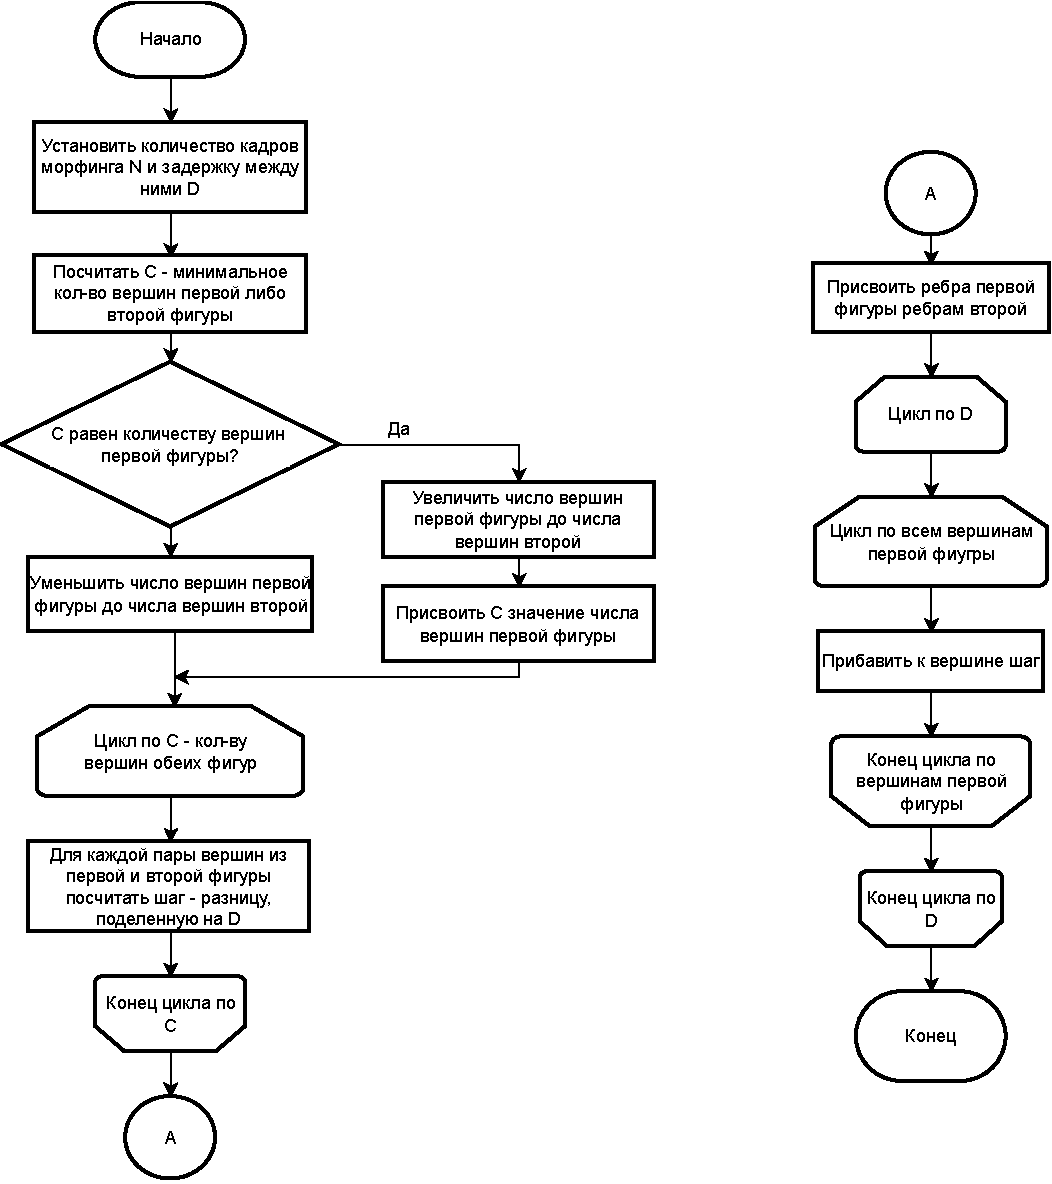
\includegraphics[scale=0.85]{images/morph_algo.pdf}
	\caption{Алгоритм морфинга двух объектов}	
	\label{fig:morph_algorithm}
\end{figure}


\section*{Выводы из конструкторского раздела}

В данном разделе была разобрана реализация выбранного алгоритма построения изображения, а также рассмотрены алгоритмы
Z-буфера, закраски по Гуро и морфинга двух фигур.

